%!TEX root = ../main.tex
\doublespacing
\chapter{The intrinsic sizes of Type III radio bursts and comparison to recent simulations.}
\label{chap:observations_vs_theory}
Recent developments in the modelling of radio waves in a turbulent corona have made predictions about source sizes that have not yet been qualitatively compared to interferometric observations. Scattering of radio waves off of density inhomogeneities in the solar corona is considered to be the dominant cause of the size and shape of radio bursts. By understanding scattering, the turbulent nature of processes that generate density inhomogeneities can be studied. Turbulence in the corona can give insight into how energy is transferred from large scale phenomena down to the microscales resulting in the million degree Kelvin temperatures that have puzzled solar physicists for decades. New models of radio wave scattering, therefore, are the first step to solving fundamental physical problems in the solar corona. However, unless the models agree with observations, their use is limited at best and as such, comparisons between models and observations are crucial. In this chapter I utilise the direct visibility fitting method described in Chapter \ref{chap:measuring_source_sizes} and apply it to 30 Type III radio bursts. It is found that these bursts have a mean size along the major and minor axis of FWHM\textsubscript{x} = 16.27 arcmin and FWHM\textsubscript{y} = 11.96 arcmin respectively. No trend of source size with respect to helioprojective angle is found, which is in direct contrast to predictions from modelling if the intrinsic size of a burst is a point source and the degree of anisotropy is high $\alpha \sim 0.3$. This study suggests that although many are in agreement, further exploration of the parameters of scattering simulations are necessary before they can be used to predict the nature of coronal density inhomogeneities.

\section{Introduction}
\label{sec:obsvtheory_intro}
The computational modelling of radio wave scattering has seen considerable development over the 50-odd years since some of the first simulations by e.g. \cite{Fokker1965} and \cite{Steinberg1971}. The theory for these early works followed from a generalisation of \cite{Chandrasekhar1952}, as was discussed in Chapter \ref{chap:theory}, and was developed to explain the observations of radio burst source size, position, directivity (power received from source in some solid angle compared to power from an isotropic source in the same solid angle) and time profile. These models considered scattering of radio photons off of density inhomogeneities in the solar corona as many small angle scatterings before the photons were allowed to travel freely. Simulations of this kind fell out of favour by the mid 1980s and remained mostly dormant until \cite{Thejappa2007} investigated the source directivity and time profiles of bursts using a different power spectrum of isotropic density inhomogeneities. In the studies by e.g. \cite{Fokker1965} and \cite{Steinberg1971}, the inhomogeneities were assumed to have a Gaussian power spectrum. However, in the intervening 30 years knowledge of turbulence in the solar corona proved this assumption to be incorrect. \cite{Coles1989} collated the results of numerous experiments to give the following description of the density inhomogeneity power spectrum. At large scales, greater than a few hundred kilometres, the spectrum is well described by the Kolmogorov spectrum with a power law index of 11/3. For scales lower than these but greater than a few kilometres, the spectrum becomes shallower and is better described with a power law index of $\sim 3$. Finally, on the smallest scales less than a few kilometres the spectrum steepens again. This steepening has been interpreted as the scale at which energy is dissipated by turbulence. \cite{Coles1989} also found that this inner scale increases with heliocentric distance. \cite{Bastian1994} expanded on this description of the density inhomogeneity power spectrum and investigated the angular broadening of radio waves sources at centimetre wavelengths.

Comparisons between the models mentioned above and observations of radio bursts have also developed over time. \cite{Stewart1972} compared the observed positions of fundamental and harmonic emission and related it to the then contemporary scattering models \citep[e.g.][]{Fokker1965,Steinberg1971,Riddle1974}. As our knowledge of solar turbulence and the power spectrum of density inhomogeneities improved so too did the instrumentation, allowing for more accurate observations of radio bursts and thus more accurate comparisons. In particular, radio interferometers such as LOFAR and the MWA have the angular resolution to investigate radio emission from both bursts \citep{Zhang2020} and the quiet sun \citep{Sharma2020}. Data from space-craft has also been used to directly compare with the model of \cite{Thejappa2007}.\cite{Krupar2018} use observations from STEREO A and B to study the time profiles of Type III radio bursts and find that these can be explained from Monte Carlo scattering code with a value for the relative r.m.s density fluctuations of $\varepsilon \sim 0.06-0.07$. This was expanded on by \cite{Krupar2020} who used data from Parker Solar probe and found that $\varepsilon$ decreased with height in the solar wind.

The latest development in the modelling of radio wave scattering is by \cite{Kontar2019}. Rather than using the small scattering angle approximation of previous work, \cite{Kontar2019} build on the work of \cite{Arzner1999} and \cite{Bian2019}. In this approach, the effect of anisotropic density inhomogeneities is treated as photon diffusion in momentum space and the Hamiltonian equations for photon position and momentum can be solved iteratively to trace a photon's path. This allows for a continuous transition from weak to strong scattering, whereas previous work is limited to regime of small angle scattering. \cite{Kontar2019} assume a spherically symmetric corona with an anisotropic distribution of electron density fluctuations, with wavenumber $\mathbf{q}$, such that $q_\parallel$ is parallel to the local radial direction. They perform Monte Carlo simulations of photons emitted from a point source at $\omega = 1.1 \omega_p(R_s)$ via fundamental plasma emission at a distance $R_s$ and an electron density from the \cite{Parker1960} density model of a spherically symmetric corona with constant temperature. The image and time profile of each burst was found by recording the arrival of each photon at some distance where scattering is considered negligible. For a radio burst that would be observed at $\sim 35$ MHz ($f_p = \omega_p/2 \pi \sim 32$ MHz) \cite{Kontar2019} find that an anisotropy factor of $\alpha = 0.3$ is necessary to explain observations of burst decay times. The effect of source location on the modelled image are also investigated and it is found that sources appear more elongated in the y direction close to the disk limb and almost circular at disk centre. This effect is less evident when an anisotropy factor of $\alpha = 0.5$ is considered.

The conclusions of \cite{Kontar2019} have not yet been qualitatively compared to observations of radio bursts. In particular, whether a relationship between the source size and its location on the solar disk exists is a easy test of the validity of recent modelling efforts. In the following sections I describe how the size of the burst in the major and minor axes (FWHM\textsubscript{x} and FWHM\textsubscript{y} respectively) are determined from LOFAR observations and how their ``aspect ratio" i.e FWHM\textsubscript{x}/FWHM\textsubscript{y}, can be used to compare the observations with recent modelling simulations.

\section{Observations}
\label{obsvtheory_observations}
During the period 04 April 2019 to 14 April 2019 a Type III radio noise storm occurred on the sun. This storm was observed in the frequency range of 20 - 80 MHz using LOFAR in both tied-array and interferometric mode. Interferometric visibilities at a frequency of 30.47 MHz from 12:00 UTC - 13:00 UTC on April 4-8 and 11-14 were obtained. During this time a large active region rotated across the solar disk. Figure \ref{fig:ar_evolve} shows how a the active region with NOAA identification number 12738 revolves onto the disk. The active region is first classified on 08 April 2019 as a unipolar sunspot under the Hale classification and evolves to a bipolar structure by 14 April 2019. The active region remains relatively simple over the duration of the observation period. Assuming Type III radio bursts occur above this active region, it offers a perfect opportunity to study the variation of source size and shape with respect to position. 

\begin{figure}[ht]
\centering
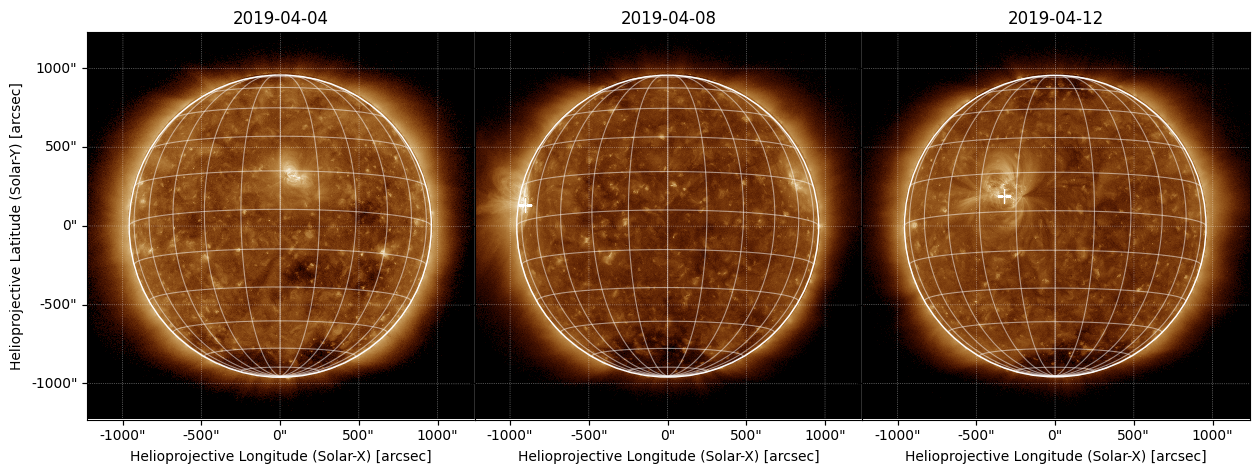
\includegraphics[width=\columnwidth]{aia193_ar_evolve.png}
\caption[Evolution of active region 12738 as it revolves around the disk.]{Evolution of active region 12738 as it revolves around the disk. Images are in the 193 \AA \ passband of AIA showing hot material in the solar corona. It is expected that Type III bursts should be centred above the active region. The left panel shows the sun on the first day of the observation where active region 12738 has not yet rotated onto disk. The middle panel shows the active region on the solar limb and is the first day where the active region is classified. The right panel shows the active region closer to the centre of the disk. }
\label{fig:ar_evolve}
\end{figure}

\section{Method}
\label{sec:obsvtheory_method}
By fitting their interferometric visibilities as described in Chapter \ref{chap:measuring_source_sizes}, the size and position of 30 Type III radio bursts over the period of 04 April 2019 to 14 April 2019 were found. The bursts were identified in LOFAR beamformed observations and their peak time determined using an automatic peak finding algorithm. Figure \ref{fig:dynamic_spectrum_070419} shows the automatically identified bursts at 30 MHz. In total, 320 bursts were identified in this way. Unfortunately, due to the strength of these bursts, the calibration of interferometric data failed for $\sim 90 \%$ of them. 30 bursts were identified manually as having successfully been calibrated and their properties fit. As well as determining the source shape and position at its peak, the area of the source over its duration was also measured. This was done by fitting a straight line to the source area over the duration of the burst, which was estimated to be 1 second before its peak and 2 seconds afterwards.

\begin{figure}[ht]
\centering
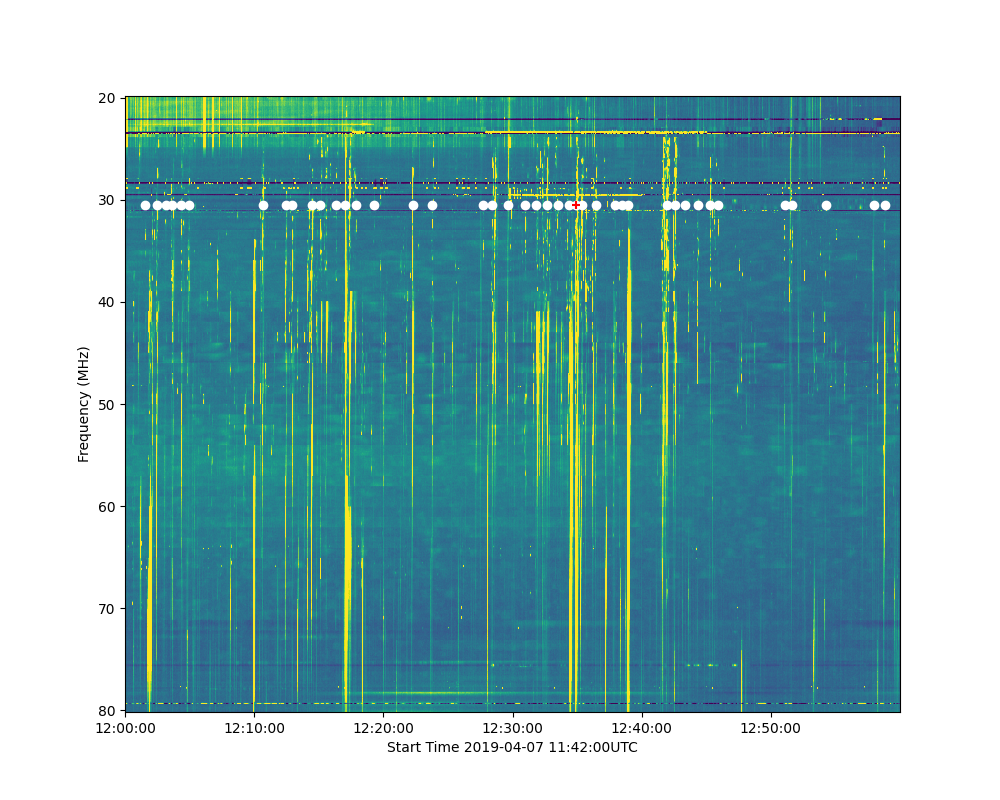
\includegraphics[width=\columnwidth]{peak_times_30MHz_2019-04-07T120000_130000.png}
\caption[Dynamic spectrum of Type III storm on 07 April 2019.]{Dynamic spectrum of Type III storm on 07 April 2019. The white dots indicate the bursts identified by an automatic peak finding algorithm, the red cross indicates the brightest burst.}
\label{fig:dynamic_spectrum_070419}
\end{figure}

\section{Results}
\label{sec:obsvtheory_results}
The parameters for all 30 fitted bursts are given in Table \ref{tab:dataset} where $I_0$ is the maximum intensity of the burst, $x_0$ and $y_0$ are the x and y  helioprojective coordinates of the burst, FWHM\textsubscript{x} and FWHM\textsubscript{y} are the burst sizes in the x and y direction and $\theta$ is the position angle of the fitted Gaussian. Each fitted type III burst is plotted in helioprojective coordinates in Figure \ref{fig:synoptic_bursts}. It is clear from the figure that most bursts share a similar size and aspect ratio despite their relatively widespread origin in relation to the Sun's disk.

\begin{figure}[ht]
\centering
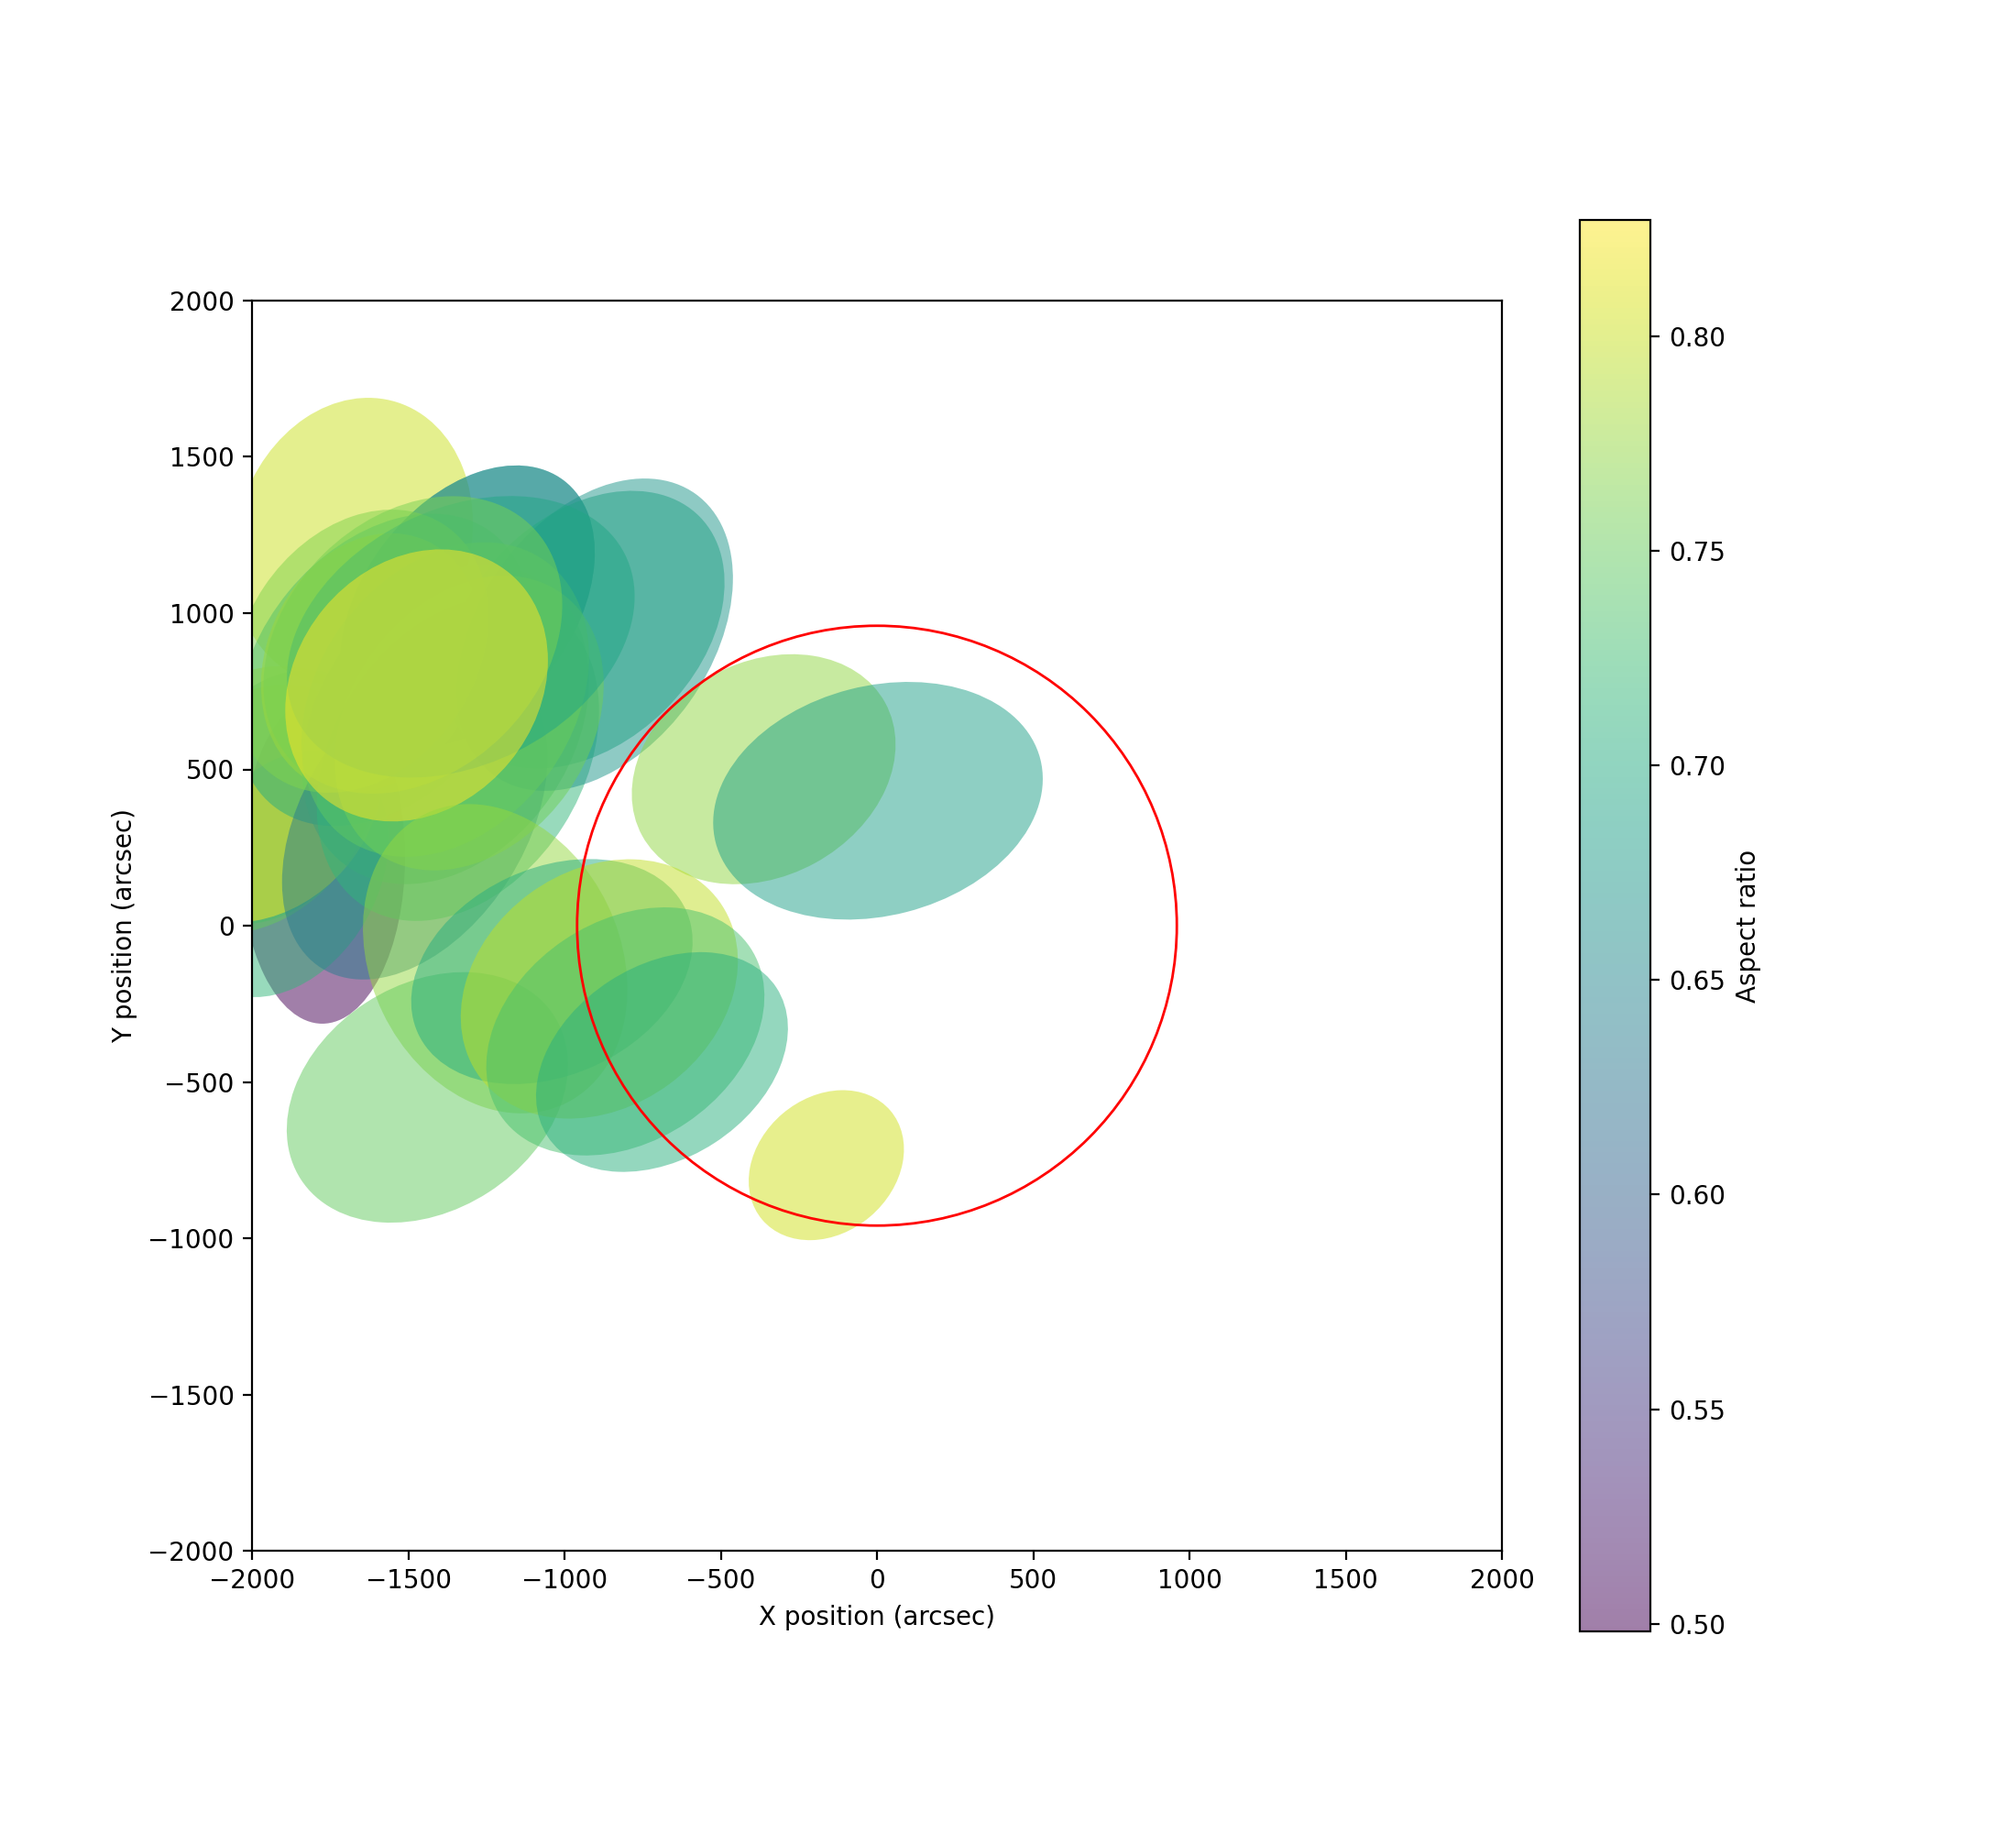
\includegraphics[width=\columnwidth]{burst_ellipses_best.png}
\caption[Plot of Type III radio bursts in helioprojecive coordinates.]{Plot of Type III radio bursts in helioprojecive coordinates. Each ellipse has the size and location determined from direct visibility fitting. The colour of each ellipse is the aspect ratio. The red circle indicates the visible solar limb. }
\label{fig:synoptic_bursts}
\end{figure}

%\begin{landscape}
\begin{table}
\centering
\caption[Table of fitted burst parameters]{Table of fitted burst parameters for each of the 30 bursts described in Section \ref{sec:obsvtheory_method}. The units in each column are given in brackets. Here $I_0$ is the maximum intensity of the burst, $x_0$ and $y_0$ are the x and y helioprojective coordinates of the burst, FWHM\textsubscript{x} and FWHM\textsubscript{y} are the burst sizes along the minor and major axes and $\theta$ is the position angle of the fitted Gaussian.}
\label{tab:dataset}
\begin{tabular}{lcccccc}
\toprule
Burst Time & $I_0$  & $x_0$ & $y_0$  & FWHM\textsubscript{x} & FWHM\textsubscript{y} & $\theta$ \\
 & (arbitrary) & (arcsec) & (arcsec) & (arcmin) & (arcmin) &  (deg) \\
\midrule
2019-04-05T12:08:08 &   90333.34 & -1772.89 &   213.66 &    8.76 &   17.58 &  -26.59 \\
2019-04-07T12:02:28 &   83782.44 & -1924.03 &   411.53 &   10.28 &   14.48 &  -56.52 \\
2019-04-07T12:04:21 &  108123.57 & -1990.30 &   372.36 &   11.29 &   14.52 &  -66.65 \\
2019-04-07T12:15:07 &  160081.88 & -1677.12 &  1228.90 &   12.48 &   15.59 &  -43.79 \\
2019-04-07T12:30:59 &  120107.74 & -1896.80 &   165.35 &   10.01 &   14.02 &  -56.17 \\
2019-04-07T12:51:39 &   47916.36 & -1979.35 &   420.47 &   12.15 &   14.72 &  -67.42 \\
2019-04-08T12:00:15 &  117196.69 & -1310.37 &  1020.77 &   11.16 &   16.93 &  -63.68 \\
2019-04-08T12:00:15 &  117196.69 & -1310.37 &  1020.77 &   11.16 &   16.93 &  -63.68 \\
2019-04-08T12:06:40 &  316272.33 & -1579.55 &   818.51 &   13.12 &   18.67 &  -65.64 \\
2019-04-08T12:08:36 &   60696.79 & -1616.67 &   840.69 &   11.28 &   14.28 &  -50.02 \\
2019-04-08T12:22:34 &  171058.10 & -1380.68 &   643.10 &   13.59 &   18.40 &  -60.80 \\
2019-04-08T12:26:53 &  111428.17 & -1479.15 &   338.94 &   11.89 &   18.69 &  -58.46 \\
2019-04-08T12:29:00 &   77443.59 & -1341.21 &   533.82 &   13.33 &   18.65 &  -58.68 \\
2019-04-08T12:34:57 &  176944.04 &  -934.63 &   947.11 &   12.09 &   17.18 &  -71.76 \\
2019-04-08T12:35:35 &  277659.44 &  -902.94 &   931.06 &   12.39 &   18.46 &  -61.85 \\
2019-04-08T12:42:59 &  119228.99 & -1653.25 &   878.17 &   12.36 &   16.18 &  -60.06 \\
2019-04-08T12:47:06 &  155057.08 & -1381.63 &   723.48 &   13.58 &   18.22 &  -62.20 \\
2019-04-08T12:48:49 &  296662.11 & -1305.03 &   648.47 &   12.83 &   16.99 &  -61.59 \\
2019-04-08T12:50:26 &  129463.84 & -1331.87 &   924.36 &   13.61 &   19.59 &  -89.59 \\
2019-04-08T12:54:34 &  207041.12 & -1485.08 &   898.27 &   13.60 &   17.91 &  -71.72 \\
2019-04-08T12:59:24 &  177435.14 & -1473.30 &   768.77 &   12.85 &   15.54 &  -65.86 \\
2019-04-11T12:56:26 &  215905.79 & -1221.80 &  -105.80 &   13.30 &   17.15 &   -0.49 \\
2019-04-12T12:00:18 &  179265.16 &  -362.53 &   500.60 &   11.41 &   14.77 &  -87.46 \\
2019-04-12T12:04:55 &  130911.18 &     3.26 &   399.69 &   12.25 &   17.88 & -101.70 \\
2019-04-12T12:14:50 &   43288.32 & -1438.75 &  -549.49 &   12.04 &   16.08 &  -83.24 \\
2019-04-12T12:39:31 &   86016.46 & -1040.30 &  -146.83 &   11.04 &   15.73 &  -91.31 \\
2019-04-12T12:49:33 &   74776.61 &  -888.52 &  -202.43 &   12.60 &   15.84 &  -79.74 \\
2019-04-12T12:51:54 &  132627.29 &  -805.26 &  -338.33 &   11.73 &   16.05 &  -82.21 \\
2019-04-12T12:53:51 &  127718.17 &  -687.98 &  -436.28 &   10.29 &   14.56 &  -83.17 \\
2019-04-13T12:30:30 &  100613.83 &  -162.06 &  -766.36 &    7.21 &    8.98 &  -75.73 \\
\bottomrule

\end{tabular}

\end{table}
%\end{landscape}
%original table with milliseconds
%\midrule
%2019-04-05T12:08:08.082 &   90333.34 & -1772.89 &   213.66 &    8.76 &   17.58 &  -26.59 \\
%2019-04-07T12:02:28.512 &   83782.44 & -1924.03 &   411.53 &   10.28 &   14.48 &  -56.52 \\
%2019-04-07T12:04:21.926 &  108123.57 & -1990.30 &   372.36 &   11.29 &   14.52 &  -66.65 \\
%2019-04-07T12:15:07.681 &  160081.88 & -1677.12 &  1228.90 &   12.48 &   15.59 &  -43.79 \\
%2019-04-07T12:30:59.620 &  120107.74 & -1896.80 &   165.35 &   10.01 &   14.02 &  -56.17 \\
%2019-04-07T12:51:39.288 &   47916.36 & -1979.35 &   420.47 &   12.15 &   14.72 &  -67.42 \\
%2019-04-08T12:00:15.636 &  117196.69 & -1310.37 &  1020.77 &   11.16 &   16.93 &  -63.68 \\
%2019-04-08T12:00:15.636 &  117196.69 & -1310.37 &  1020.77 &   11.16 &   16.93 &  -63.68 \\
%2019-04-08T12:06:40.505 &  316272.33 & -1579.55 &   818.51 &   13.12 &   18.67 &  -65.64 \\
%2019-04-08T12:08:36.604 &   60696.79 & -1616.67 &   840.69 &   11.28 &   14.28 &  -50.02 \\
%2019-04-08T12:22:34.290 &  171058.10 & -1380.68 &   643.10 &   13.59 &   18.40 &  -60.80 \\
%2019-04-08T12:26:53.834 &  111428.17 & -1479.15 &   338.94 &   11.89 &   18.69 &  -58.46 \\
%2019-04-08T12:29:00.334 &   77443.59 & -1341.21 &   533.82 &   13.33 &   18.65 &  -58.68 \\
%2019-04-08T12:34:57.353 &  176944.04 &  -934.63 &   947.11 &   12.09 &   17.18 &  -71.76 \\
%2019-04-08T12:35:35.437 &  277659.44 &  -902.94 &   931.06 &   12.39 &   18.46 &  -61.85 \\
%2019-04-08T12:42:59.698 &  119228.99 & -1653.25 &   878.17 &   12.36 &   16.18 &  -60.06 \\
%2019-04-08T12:47:06.994 &  155057.08 & -1381.63 &   723.48 &   13.58 &   18.22 &  -62.20 \\
%2019-04-08T12:48:49.167 &  296662.11 & -1305.03 &   648.47 &   12.83 &   16.99 &  -61.59 \\
%2019-04-08T12:50:26.643 &  129463.84 & -1331.87 &   924.36 &   13.61 &   19.59 &  -89.59 \\
%2019-04-08T12:54:34.610 &  207041.12 & -1485.08 &   898.27 &   13.60 &   17.91 &  -71.72 \\
%2019-04-08T12:59:24.856 &  177435.14 & -1473.30 &   768.77 &   12.85 &   15.54 &  -65.86 \\
%2019-04-11T12:56:26.514 &  215905.79 & -1221.80 &  -105.80 &   13.30 &   17.15 &   -0.49 \\
%2019-04-12T12:00:18.153 &  179265.16 &  -362.53 &   500.60 &   11.41 &   14.77 &  -87.46 \\
%2019-04-12T12:04:55.480 &  130911.18 &     3.26 &   399.69 &   12.25 &   17.88 & -101.70 \\
%2019-04-12T12:14:50.568 &   43288.32 & -1438.75 &  -549.49 &   12.04 &   16.08 &  -83.24 \\
%2019-04-12T12:39:31.661 &   86016.46 & -1040.30 &  -146.83 &   11.04 &   15.73 &  -91.31 \\
%2019-04-12T12:49:33.963 &   74776.61 &  -888.52 &  -202.43 &   12.60 &   15.84 &  -79.74 \\
%2019-04-12T12:51:54.388 &  132627.29 &  -805.26 &  -338.33 &   11.73 &   16.05 &  -82.21 \\
%2019-04-12T12:53:51.493 &  127718.17 &  -687.98 &  -436.28 &   10.29 &   14.56 &  -83.17 \\
%2019-04-13T12:30:30.763 &  100613.83 &  -162.06 &  -766.36 &    7.21 &    8.98 &  -75.73 \\
%\bottomrule


The size of each burst, is plotted against the distance from the disk centre in the x and y direction in Figure \ref{fig:fwhm_comp}. There is no obvious trend towards bigger/smaller bursts with increasing distance from disk centre and, most strikingly, in direct contrast to the prediction by \cite{Kontar2019} there is no trend in the aspect ratio of the bursts, which is expected to trend towards 1 near disk centre and $< 1$ near the limb. Figure \ref{fig:fwhm_hist} shows a histogram of FWHM\textsubscript{x} and FWHM\textsubscript{y}in the range of 6 to 20 arcmins. The mean size of the bursts is indicated by a vertical grey dashed line and is $11.96$ arcmin for FWHM\textsubscript{x} and $16.27$ arcmin for FWHM\textsubscript{y}. The mean aspect ratio of the bursts is $\sim 0.74$.

\begin{figure}[ht]
\centering
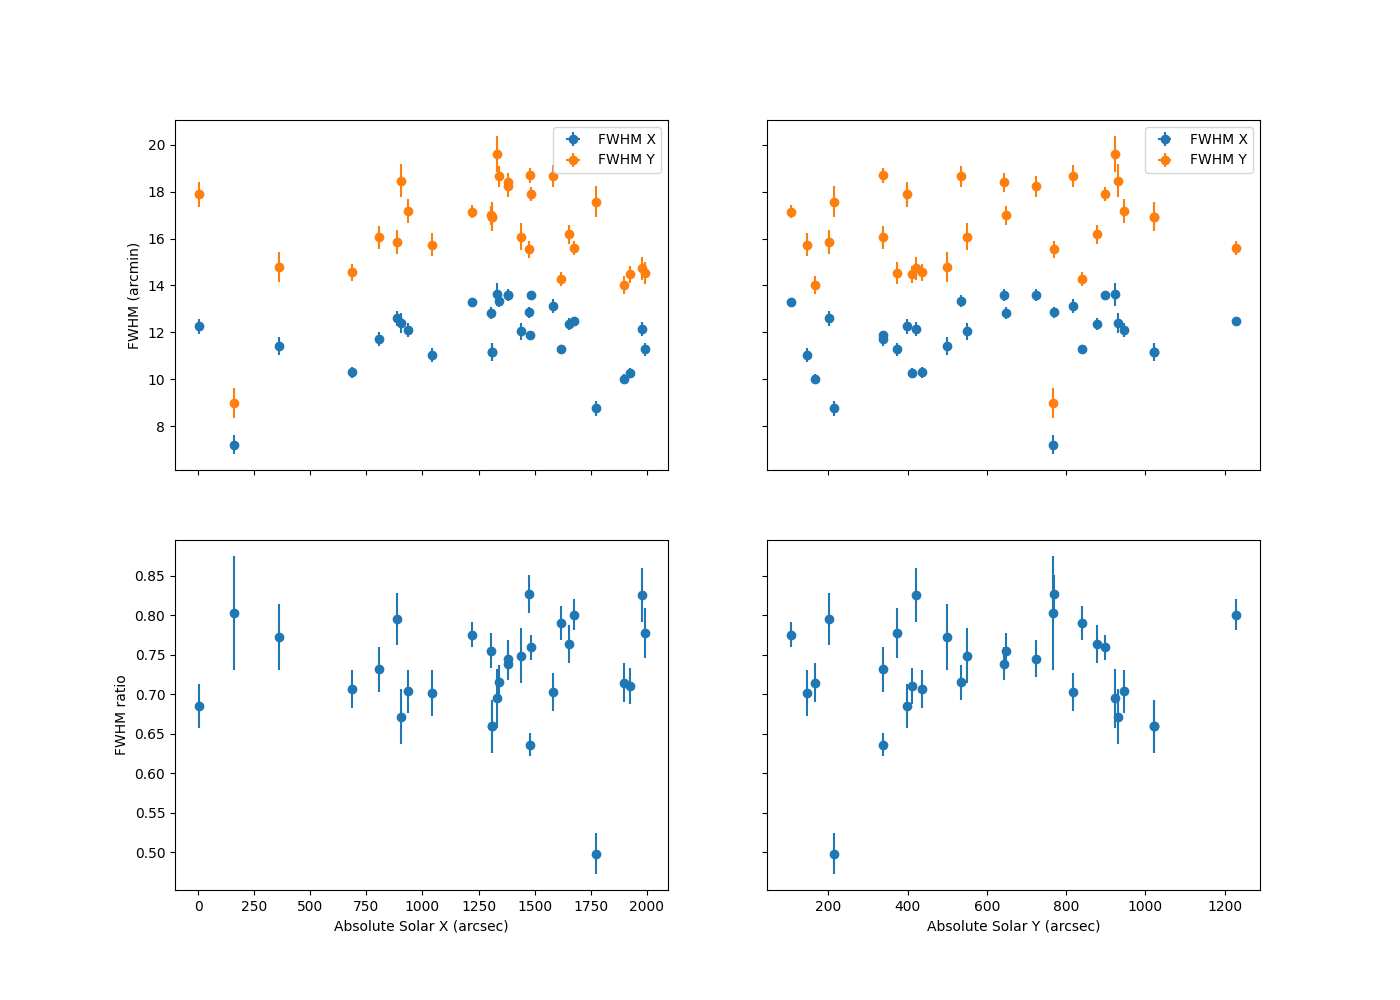
\includegraphics[width=\columnwidth]{fwhm_comparison.png}
\caption[Directly fitted Type III burst sizes as a function of position relative to disk centre.]{A comparison of the directly fitted Type III burst sizes and their location relative to the disk centre in the x and y direction. Top row, FWHM in x (blue) and y (orange) as a function of their distance from the disk centre in the x (left) and y (right) direction. Bottom row, same as above except showing the ``aspect ratio" of each burst.}
\label{fig:fwhm_comp}
\end{figure}

\begin{figure}[ht]
\centering
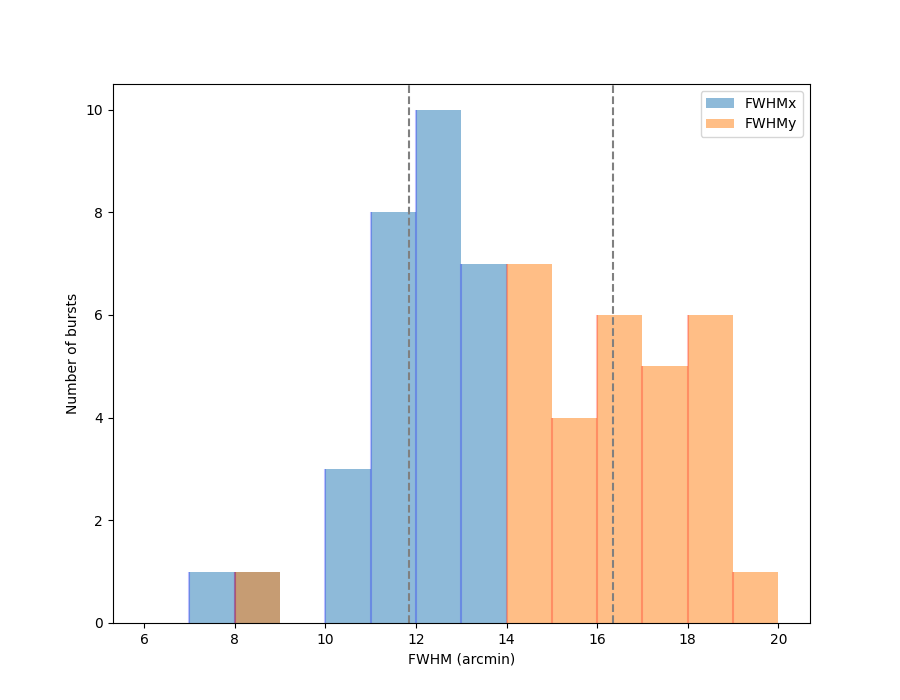
\includegraphics[width=\columnwidth]{burst_fwhm_histogram.png}
\caption[Histogram of type III burst sizes.]{Histogram of type III burst sizes. Bins are 1 arcmin wide and the vertical dashed lines indicate the mean value for FWHM\textsubscript{x} (blue) and FWHM\textsubscript{y} (red).}
\label{fig:fwhm_hist}
\end{figure}

\begin{figure}[ht]
\centering
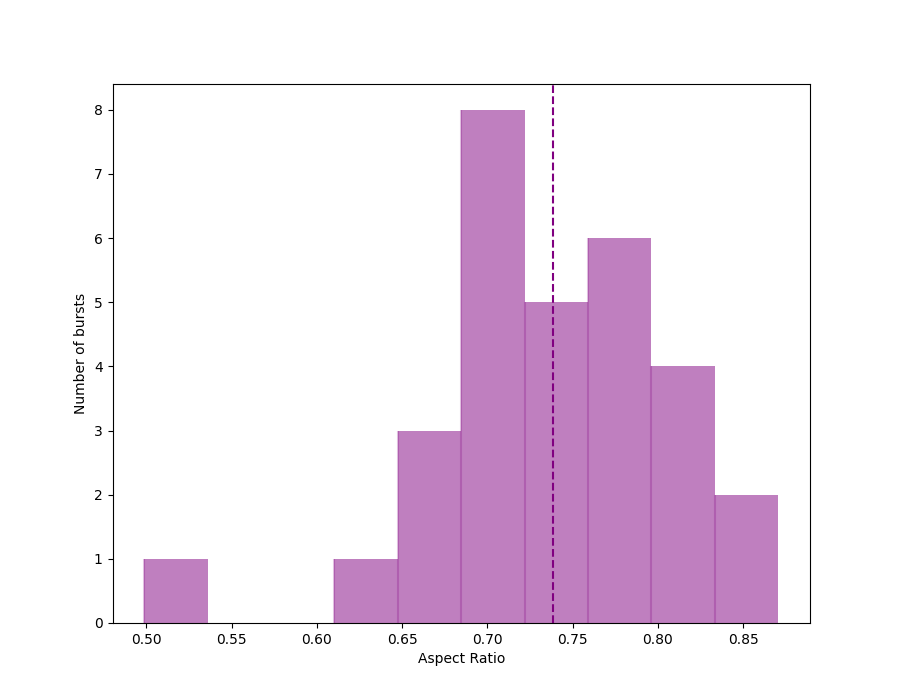
\includegraphics[width=\columnwidth]{burst_fwhm_ratio_histogram.png}
\caption[Histogram of type III burst aspect ratios.]{Histogram of type III burst aspect ratios. The vertical purple dashed line indicates the mean value for the aspect ratio FWHM\textsubscript{x}/FWHM\textsubscript{y}.}
\label{fig:fwhm_ratio_hist}
\end{figure}

The relative angle of each burst i.e. the angle between the minor axis of the burst and a line from its centre to (0,0) in helioprojective coordinates, is plotted as a histogram in Figure \ref{fig:rel_ang_hist}. These are peaked in the $-20^\circ - 0^\circ$ bin and have a mean of $-18.33^\circ$.

\begin{figure}[ht]
\centering
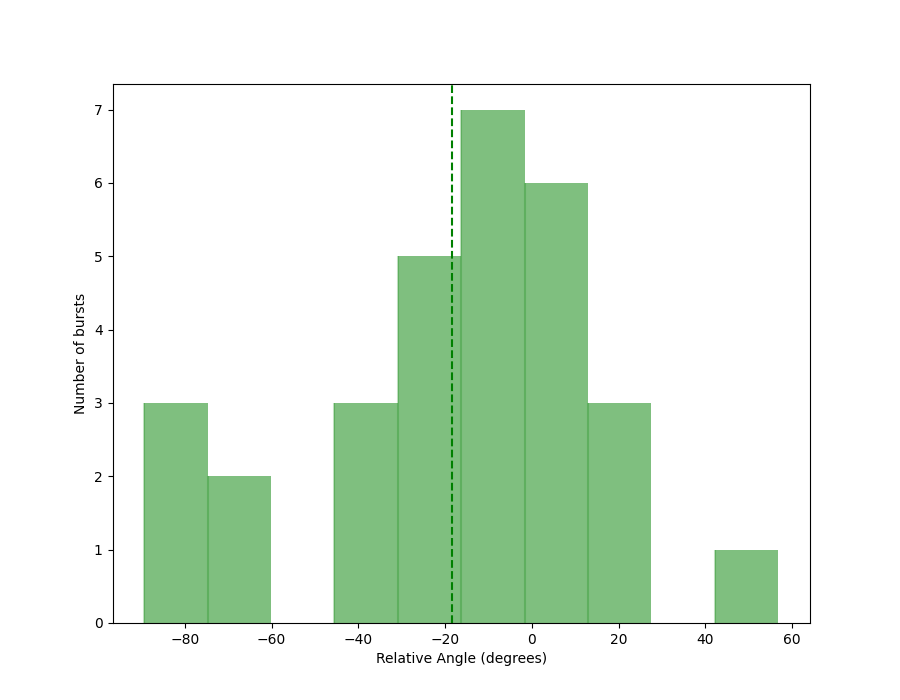
\includegraphics[width=\columnwidth]{burst_relative_angle_histogram.png}
\caption[Histogram of type III burst relative angles.]{Histogram of type III burst relative angles. The vertical green dashed line indicates the mean value for the angle between the minor axis of the burst and a line joining its centre to (0,0).}
\label{fig:rel_ang_hist}
\end{figure}

\section{Discussion}
\label{sec:obsvtheory_discussion}
The observed source sizes of Type III bursts are largely consistent with previous observations at similar frequencies in both interferometric and tied-array observations \citep{Kontar2017, Zhang2020}. In particular, the mean of the size in the major and minor axes is in agreement a previous measurement using the visibility fitting method \citep{Murphy2021}. As well as this, all 30 of the fitted bursts have an aspect ratio (defined above) of less than 1, which is suggestive of preferential scattering in a particular direction \citep{Anantharamaiah1994, Bastian1994}. The peaked distribution of relative angles in Figure \ref{fig:rel_ang_hist} is further evidence for alignment along a preferred direction. If this direction were radial one would expect a peak around $0^\circ$ however here a mean value of $-18.33^\circ$ is observed. A thorough examination of the magnetic field structure of the active region could determine whether the bursts are well aligned perpendicular to the magnetic field lines as has been observed in the solar wind \citep{Anantharamaiah1994, SasikumarRaja2016}.

There is one major deviation between the model of scattering through anisotropic density fluctuations in a spherically symmetric corona and these results. \cite{Kontar2019} predict that, for a point source, the aspect ratio of a radio burst should decrease with increasing heliocentric angle, i.e. distance away from the disk centre along the solar equator. However, as shown in Figure \ref{fig:fwhm_comp}, no such trend is evident in the data.  The simplest, and perhaps most appropriate, answer to why this is the case is mentioned in the discussion of \cite{Kontar2019}. Since their work only analyses the path of photons from a point source, it is possible that Type III (and other) radio bursts have an intrinsic source size. The total observed size then can be considered as the intrinsic size and the size due to scattering of a point source added in quadrature FWHM\textsubscript{total} = (FWHM\textsuperscript{2}\textsubscript{intrinsic} + FWHM\textsuperscript{2}\textsubscript{scattering})$^{1/2}$. Therefore, no trend in source sizes could suggest an intrinsic size greater than the size due to scattering. An alternative explanation could be that the anisotropy is much less than \cite{Kontar2019} suggest, perhaps having a value closer to $\alpha = 0.5$. 

The histogram of burst sizes in Figure \ref{fig:fwhm_hist} shows that the minor size of the bursts are peaked around the mean whereas the major size shows no peak. It stands to reason that the source size in the minor direction undergoes less scattering, therefore retaining its intrinsic size, than in the major direction where the size distribution is almost random.

Perhaps a more damning indictment for all scattering models comes when one relaxes the assumption of a spherically symmetric solar corona that is constant in time.  If, as is widely accepted, radio burst generation is concentrated in open magnetic field lines above the active region seen in Figure \ref{fig:ar_evolve} then the spectrum of density inhomogeneities is sure to change as the active region evolves. The time scale for this change is clearly less than the order of a few days, otherwise the trend in aspect ratio should be observed in Figure \ref{fig:fwhm_comp}. A lower limit on this time scale is more elusive. Bursts observed over the course of one hour on a given day all share a similar size, orientation and aspect ratio which gives a lower limit of at least one hour. Thus it is reasonable to assume that the power spectrum of density inhomogeneities is constant on the order of a few hours but not for time scales over a number of days. The exact change to the power spectrum during this time remains unknown but is undoubtedly linked to magnetic flux emergence in the active region and it is likely that the assumption of constant $\varepsilon$ is also incorrect and that either the level r.m.s fluctuations change or the actual electron density of the emitting region changes.

It is a fair criticism that absolute x positions in the range 0 - 1000 arcsec and absolute y positions in the range 0 - 200 arcsec are under sampled compared to the dense cluster of bursts observed around -1500 arcsec, 750 arcsec. The reason for this discrepancy, while not justifying it, is because of poor calibration of the interferometric visibilities as the radio noise storm became more intense. This coincided with the active region rotating to the centre of the solar disk and thus poor sampling in this region. That said, I think the discussion above still stands and I'll tell you why. Repeating the above analysis with bursts fitted even though there is poor calibration returns much the same result although with greater scatter and error, as one might expect. Therefore, even though the bursts shown in this chapter may not fully sample the space, they are properly representative of the overall picture.

\section{Conclusion}
In this chapter I outlined the development of scattering models for radio waves in the solar corona from seminal works to modern day advancements. I also stated the importance that comparisons between these models and contemporary observations. I then detail the observation of hundreds of Type III radio bursts during a radio noise storm over the period 04 April 2019 to 14 April 2019. Using LOFAR interferometric visibilities at $\sim 30$ MHz and a method similar to \cite{Murphy2021} I fit 30 of the calibrated bursts to determine their size and shape. I find that Type III radio bursts have a mean size in the minor and major axis of $11.96$ arcmin for and $16.27$ arcmin respectively and a mean aspect ratio of 0.74. No trend in aspect ratio with respect to burst location is evident in the observations and as such, I attribute this to the intrinsic size of Type III radio bursts being greater than the size due to scattering. The relative angle between the minor axis of each burst and a radial line from the centre of the sun to its centre has a mean value of $-18.33^\circ$ and indicates preferential orientation, probably to the local magnetic field lines. Using the mean values achieved as a typical intrinsic size agrees well with previous observations with LOFAR in both interferometric and tied-array images at similar frequencies.

